\documentclass{article}
\usepackage[letterpaper,top=2cm,bottom=1.5cm,left=2cm,right=2cm,marginparwidth=1.75cm]{geometry}
\usepackage[english]{babel}
\usepackage{tcolorbox}
\usepackage{xcolor}
\usepackage[pdftex]{hyperref}
\usepackage{fancyhdr}
\usepackage{algorithm}
\usepackage{algpseudocode}
\usepackage{listings}
\usepackage{amsthm}
\usepackage{amsmath}

\hypersetup{
    colorlinks=true,
    linkcolor=black,
    urlcolor=black,
}

\definecolor{codegreen}{rgb}{0,0.6,0}
\definecolor{codegray}{rgb}{0.5,0.5,0.5}
\definecolor{codepurple}{rgb}{0.58,0,0.82}
\definecolor{backcolour}{rgb}{0.95,0.95,0.92}

\lstset{language=C++,
        backgroundcolor=\color{backcolour},
        commentstyle=\color{codegreen},
        keywordstyle=\color{magenta},
        numberstyle=\tiny\color{codegray},
        stringstyle=\color{codepurple},
        basicstyle=\ttfamily\footnotesize,
        breakatwhitespace=false,
        breaklines=true,
        captionpos=b,
        keepspaces=true,
        numbers=left,
        numbersep=5pt,
        showspaces=false,
        showstringspaces=false,
        showtabs=false,
        tabsize=2
}

\title{LAB 1 ASSIGNMENT}
\author{Sanz Alonso Jesús, Prieto Páez Agustín}
\date{\today}

\begin{document}
\pagestyle{fancy}
\fancyhead[R]{Sanz, Prieto}
\fancyfoot[C]{\thepage}
\maketitle
\tableofcontents

\section{Description}
We have to implement four different kind of state space search algorithms in order to reach a goal state. We must implement \textbf{Breadth-First Search}, \textbf{Depth-First Search}, \textbf{A*} and \textbf{Best-First Search} (Heuristics).

\section{Statistical Analysis}
\subsection{Description of the algorithm}
\subsubsection{Base solution}

\begin{itemize}
	\item Rough description of the main ideas of the algorithm to solve this problem as it would
	      be explained to a class mate that does not know what a backtracking programming way of solving problems is.

	      \textbf{Answer}:\quad The algorithm aims to distribute goods among a limited number of trucks, ensuring
	      that each truck's weight limit is not exceeded. It begins by checking if such a distribution is feasible.
	      If so, it sorts the goods by weight and recursively attempts to place them in trucks, backtracking when necessary.
       
\section{Algorithmic complexity}
	\item Formal description of the backtracking programming algorithm that solves the problem, so previously
	      identifying the key elements we have been working with in class:
	      \begin{itemize}
		      \item \textbf{Solution Data Type}: The solution is a mapping of goods to trucks, where each truck's weight limit
		            is not exceeded.
		      \item \textbf{Exhaustivity}: The algorithm explores all possible combinations of assigning goods to trucks until
		            a feasible solution is found or all combinations are exhausted.
		      \item \textbf{Dead Node Condition (Backtracking)}: If placing a good in a truck would exceed its capacity, the
		            algorithm backtracks to the previous state and explores other possibilities.
		      \item \textbf{Live Node Condition}: If the current assignment of goods to trucks does not exceed any truck's
		            capacity and there are goods remaining, the algorithm continues exploring further assignments.
		      \item \textbf{Solution Node Condition}: If all goods are successfully assigned to trucks without exceeding
		            any capacity, a solution is found.
	      \end{itemize}
\end{itemize}
 \begin{center}
		      \begin{figure}[!ht]
			      \centering
			      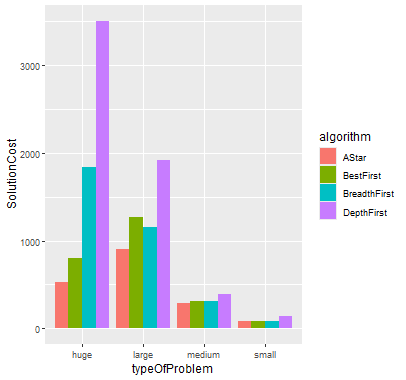
\includegraphics[scale=0.7]{images/costOfAlgorithmsInEachGroupOfProblems.png}
			      \caption{Cost of each strategy used for problems with different dimensions.}
			      \label{fig:complexity-graph-comparison}
		      \end{figure}
	      \end{center}

\subsubsection{Optimization}
The following optimizations have been applied to improve the efficiency of the backtracking algorithm:
\begin{enumerate}
	\item \textbf{Feasibility Check}: Before starting the backtracking process, a feasibility check is performed to determine if it's even possible to distribute all goods among the given number of lorries without exceeding the capacity of each lorry or the budget constraint.

	\item \textbf{Sorting}: The weights of goods are sorted in non-increasing order using the \texttt{quickSort} function. Sorting the weights allows the algorithm to try heavier goods first, potentially reducing the search space.

	\item \textbf{Pruning}: During the backtracking process, if a particular combination of goods and lorries exceeds the load capacity of any lorry, that branch of the search tree is pruned. Similarly, if the cost exceeds the budget constraint, the branch is also pruned. This avoids exploring solutions that are guaranteed to be invalid.

	\item \textbf{Array to Track Goods Assignment}: An array \texttt{selected[NUM\_LORRIES][n]} is used to keep track of which goods are assigned to which lorries. This allows the algorithm to print out the weights assigned to each lorry once a valid solution is found.

	\item \textbf{Avoiding Redundant Permutations}: When checking if a lorry has a load capacity of 0, it breaks the loop to avoid redundant permutations. This helps in reducing unnecessary computations.
\end{enumerate}

\subsection{Pseudocode}
\begin{algorithm}
	\caption{Main Algorithm}
	\label{algo:main}
	\begin{algorithmic}[1]
		\Function{Main}{}
		\State Create DataBase
		\For{$i \gets small \textbf {to}  huge$}
			\For{$i \gets 0 \textbf{to} numberFiles-1$}
				\State \textbf{read} $problemNameFile$
				\State \textbf{declare} $problem$
				\State \textbf{declare} $searchStrategy$
				\State \Call{Search}{}
				\State write results on the DataBase
			\EndFor
		\EndFor
		\EndFunction
	\end{algorithmic}
\end{algorithm}

\begin{algorithm}
	\caption{Search Algorithm}
	\label{algo:search}
	\begin{algorithmic}[1]
		\Function{search}{$StrategyToUse$}
		\If{$index = n$}
		\State \textbf{return} true
		\EndIf
            \State$i \gets index\%3$
		\For{$j \gets 0 \ \textbf{to} \  
    NUM\_LORRIES - 1, \ j \gets j+1$}
		\If{$lorries[i] + weights[index] \leq max\_capacity$}
		\State $lorries[i] \gets lorries[i] + weights[index]$
		\If{\Call{CanPlaceGoodsSnake}{$weights[], lorries[], index + 1, n, max\_capacity, selected[][]$}}
            \State $selected[i][index] \gets true$
		\State \textbf{return} true
		\EndIf
		\State $lorries[i] \gets lorries[i] - weights[index]$
		\EndIf
		\If{$lorries[i] = 0$}
		\State \textbf{break}
		\EndIf
  \State$ i \gets INCREMENT\_SNAKE(i,index)$
		\EndFor
		\State \textbf{return} false
		\EndFunction
	\end{algorithmic}
\end{algorithm}
\begin{algorithm}
	\caption{FeasibilityCheck Algorithm}
	\label{algo:feasibilitycheck}
	\begin{algorithmic}[1]
		\Function{FeasibilityCheck}{$weights[], n$}
		\State $sum \gets 0$
		\For{$,n \  \textbf{and} \ sum \leq NUM\_LORRIES \times max\_capacity \ \textbf{and} \ weights[n - 1] \leq max\_capacity \ \textbf{and} \ sum \times cost\_per\_kg \leq budget,$}
            \State $n \gets n - 1$
            \State $sum \gets sum + weights[n]$
            \EndFor
		\State \textbf{return $\textbf{not} \ n \ \textbf{and} \  sum \leq NUM\_LORRIES \times max\_capacity \ \textbf{and} \   sum \times cost\_per\_kg \leq budget $}
		\EndFunction
	\end{algorithmic}
\end{algorithm}


\begin{algorithm}
	\caption{CanPlaceGoodsBalancedSum Algorithm}
	\label{algo:canplacegoodsbalancedsum}
	\begin{algorithmic}[1]
		\Function{CanPlaceGoodsBalancedSum}{$weights[], lorries[], index, n, max\_capacity, selected[][]$}
		\If{$index = n$}
		\State \textbf{return} true
		\EndIf
            \State $Define\ \textit{start}\ and\ \textit{increment}\ as\ integers$
            \If{$lorries[0] \leq lorries[1] \And lorries[0] \leq lorries[2]$}
            \State $start \gets 0$
            \If{$lorries[1] \leq lorries[2]$}
            \State $increment \gets 1 $
            \Else \State $increment \gets -1$
            \EndIf
            \Else \If{$lorries[1] \leq lorries[0] \And lorries[1] \leq lorries[2]$}
            \State $start \gets 1$
            \If{$lorries[0] \leq lorries[2]$}
            \State $increment \gets 1 $
            \Else \State $increment \gets -1$
            \EndIf
            \Else \State $start \gets 2$
            \If{$lorries[0] \leq lorries[1]$}
            \State $increment \gets 1 $
            \Else \State $increment \gets -1$
            \EndIf
            \EndIf
            \EndIf
            \State $i \gets start$  
		\For{$ j \gets 0$ \textbf{to} $NUM\_LORRIES - 1, \ j \gets j+1 $}
            
		\If{$lorries[i] + weights[index] \leq max\_capacity$}
		\State $lorries[i] \gets lorries[i] + weights[index]$
		\If{\Call{CanPlaceGoodsBalancedSum}{$weights[], lorries[], index + 1, n, max\_capacity, selected[][]$}}
            \State $selected[i][index] \gets true$
		\State \textbf{return} true
		\EndIf
		\State $lorries[i] \gets lorries[i] - weights[index]$
		\EndIf
		\If{$lorries[i] = 0$}
		\State \textbf{break}
		\EndIf
  \State $i \gets INCREMENT\_SUM(i,increment)$
		\EndFor
		\State \textbf{return} false
		\EndFunction
	\end{algorithmic}
\end{algorithm}

 Note: On \textbf{Algorithm 3} \textit{FeasiblityCheck Algorithm} we have got an implicit conversion from integer, \textit{n}, to boolean. We must mention that 0 is false, true otherwise.

\subsection{Complexity analysis}
\begin{itemize}
	\item Analysis of the \textbf{computational complexity} of the algorithm in terms of the number of operations
	      executed by the algorithm as a function of the input size \textit{n}.

	      \textbf{Answer}:\quad The backtracking algorithm's complexity is analyzed based on the number of operations it executes, which is a function of the input size \(n\), the maximum load capacity of the lorries \textit{MAX\_CAPACITY}, and the maximum number of lorries \textit{NUM\_LORRIES}. The algorithm consists of several key components, each contributing to the overall complexity as follows:

	      \begin{enumerate}
		      \item \underline{Sorting the Weights:} The algorithm begins by sorting the weights in non-increasing order.
		            This sorting operation typically takes \(O(n \log n)\) time using efficient sorting algorithms like quicksort or mergesort.

		      \item \underline{Feasibility Check:} Before initiating the backtracking process, a feasibility check is performed to determine
		            if it's possible to distribute all goods among the given number of lorries without exceeding their capacities. This check involves iterating through the weights and ensuring that the sum of weights does not exceed \textit{NUM\_LORRIES} times \textit{MAX\_CAPACITY}. This operation has a complexity of \(O(n)\).

		      \item \underline{Backtracking Process:} The core of the algorithm is the backtracking process, where it recursively
		            explores all possible combinations of assigning goods to lorries. At each step, it tries to place the current good in each lorry,
		            branching into multiple recursive calls. The maximum depth of the recursion tree is bounded by the number of goods \(n\),
		            and at each level, there are \(O(\textit{NUM\_LORRIES})\) choices. Therefore, the time complexity of the backtracking
		            process is \(O(\textit{NUM\_LORRIES}^n)\).

		      \item \underline{Solution Output:} After finding a feasible distribution, the algorithm outputs the assigned goods for each lorry along with the total cost. This operation involves iterating through the selected goods and has a complexity of \(O(n)\).
	      \end{enumerate}

	      Considering these components, the overall complexity of the backtracking algorithm is influenced primarily by the backtracking process, which has a complexity of \(O(\textit{NUM\_LORRIES}^n)\). Additionally, the sorting operation contributes \(O(n \log n)\), and the feasibility check and solution output operations contribute \(O(n)\) each.

	      Thus, the total complexity of the algorithm can be described as:
	      \[
		      T(n, \textit{NUM\_LORRIES} = 3) \in O(n + n \log n + 3^n) \approx O(3^3)
	      \]
	      where \(n\) represents the number of goods, \textit{MAX\_CAPACITY} is the maximum load capacity of the lorries, and \textit{NUM\_LORRIES} is the maximum number of lorries.
\item{Description of Quicksort Time Complexity on Average Case}

\[
T(n)=O(n)+2T\left(\frac{n}{2}\right)
\]

\[
n=2^i
\]

\[
2^i-2\cdot2^{(i-1)}=2^i
\]

\[
r^i-2\cdot r^{(i-1)}=2^i
\]

\[
r-2=0
\]

From left hand side we have got that \(r=2\) and \(\alpha=1\).

From the right hand side we have got that \(r=2\) and \(\alpha=1\).

In brief, \(r=2\) and \(\alpha=2\).

So that we can construct our expression with degree \(\alpha-1\).

\[
T(2^i)=2^i \cdot A+B \cdot 2^i \cdot i
\]

On variable change,

\[
T(n)=(A+B \cdot \log_2 n)\cdot n
\]

Where \(\Omega(n)\) and \(O(n\log n)\)


	\item Test of the algorithm with increasing values of \textit{n} and analysis of the time taken by the algorithm (\textit{CPU time}).

	      Bear in mind that the specific time taken by the algorithm may vary depending on the machine used to run the code
	      and the \textit{GCC compiler} optimization settings. We must disable the optimization flag to get the real time taken by the algorithm,
	      otherwise the compiler will optimize the code and, therefore, the graph of \textit{CPU time} will not be a representative approximation.
	      \begin{itemize}
		      \item GPU: \textit{AMD Ryzen 5 3500U with Radeon Vega Mobile Gfx}
		      \item GCC compiler: \textit{gcc (Ubuntu 11.4.0-1ubuntu1~22.04) 11.4.0}
		      \item GCC optimization flag: \textit{\#pragma GCC optimize("O0")} (GCC compiler optimization disabled)
	      \end{itemize}

	      \begin{lstlisting}[language=C++, caption = Optimization settings and time measurement., label=lst:code4]
#include <time.h>
#pragma GCC optimize("O0")

if (!feasibilityCheck(weights, n, LOAD_CAPACITY, NUM_LORRIES, BUDGET, COST_PER_KG))		// O(n)
{
    printf("\nIt's not possible to distribute all goods in 3 lorries without exceeding the capacity of 20 Tm each.\n");
}
else
{
    qsort(weights, n, sizeof(int), compare);                           		// O(nlogn)
    bool result = canPlaceGoods(weights, lorries, 0, n, LOAD_CAPACITY); 	// O(3^n)
}
    
end = clock();
cpu_time_used = ((double)(end - start)) / CLOCKS_PER_SEC * 1000.0;
\end{lstlisting}

	      \begin{center}
		      \begin{figure}[!ht]
			      \centering
			      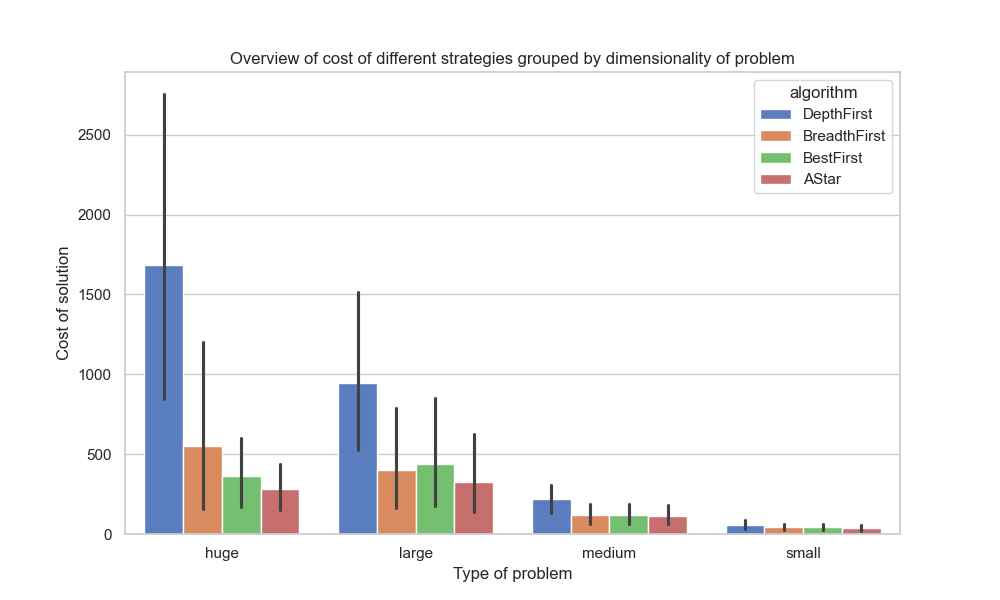
\includegraphics[scale=0.7]{images/mi_grafica.png}
			      \caption{Graphic showing the cost of each strategy compared within each dimension of the problems.}
			      \label{fig:complexity-graph}
		      \end{figure}
	      \end{center}
        \begin{center}
		      \begin{figure}[!ht]
			      \centering
			      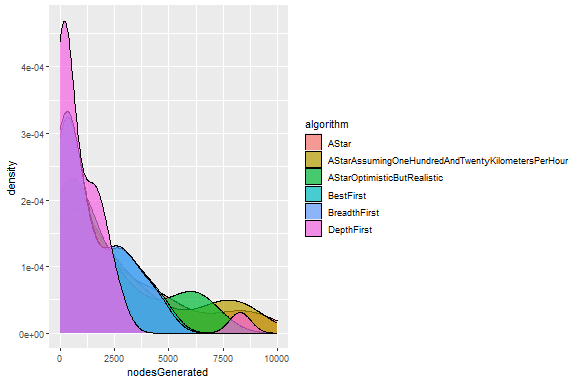
\includegraphics[scale=0.7]{images/nodesGeneratedOnDifferentStrategies.png}
			      \caption{Density graphic showing the nodes generated of each Search Strategy.}
			      \label{fig:complexity-graph}
		      \end{figure}
	      \end{center}

	      \begin{center}
		      \begin{figure}[!ht]
			      \centering
			      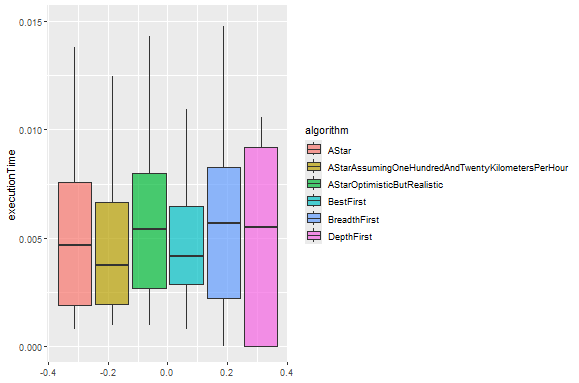
\includegraphics[scale=0.7]{images/differentAlgorithmsExecutionTime.png}
			      \caption{Negative execution time for A* strategy on huge dimension of problems.}
			      \label{fig:complexity-graph-comparison}
		      \end{figure}
	      \end{center}

	\item \textbf{Conclusion}: The empirical CPU time used by the optimized backtracking algorithm exhibits an unexpected trend
	      when compared to the predicted exponential complexity of \( O(3^n) \). The graph suggests a performance that is closer to
	      linear, possibly due to effective optimizations. This discrepancy between theoretical and observed complexity underscores
	      the impact of practical enhancements in algorithm implementation. Assuming the number of operations is proportional to the
	      number of items, the empirical complexity could be approximated as \( O(n) \), a significant improvement over the theoretical expectation.
\end{itemize}
\begin{center}
		      \begin{figure}[!ht]
			      \centering
			      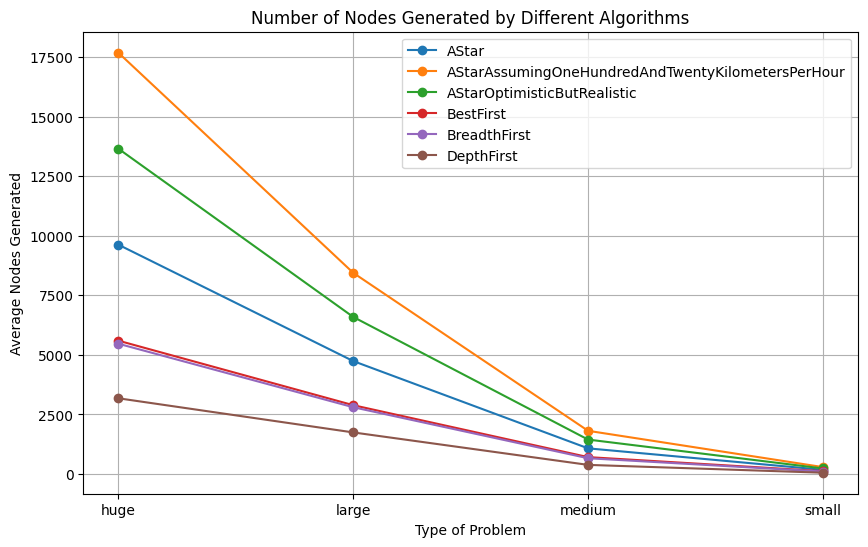
\includegraphics[scale=0.7]{images/nodes_generated_comparison.png}
			      \caption{Average Nodes Generated on different search strategies across problems with different dimensionality.}
			      \label{fig:complexity-graph-comparison}
		      \end{figure}
	      \end{center}
\end{document}